\documentclass{report}
\usepackage[utf8]{vietnam}
\usepackage[14pt]{extsizes}
\usepackage{amsmath,amsfonts,amsthm,graphicx}
\usepackage[spaces,hyphens]{url}
\usepackage{geometry}
\usepackage{tikz,tcolorbox}
\usepackage{hyperref}
\usepackage{setspace}
\usepackage{fancyvrb}
\usepackage{fancyhdr,lastpage}
\usepackage{lipsum}
\usepackage{setspace}
\onehalfspacing
\pagestyle{fancy}
\lhead{Nhóm 33}
\rhead{Trường Đại học Công nghệ}
\geometry{
 a4paper,
 total={170mm,257mm},
 left=20mm,
 top=20mm,
}
\title{\textbf{\Large BÁO CÁO\\ GIỚI THIỆU VỀ MICROSOFT COPILOT}}
\author{Nhóm 33\\ Trường Đại học Công nghệ - Đại học Quốc gia Hà Nội}
\begin{document}
\maketitle
\chapter*{Tóm tắt}
Sự bùng nổ của công nghệ trí tuệ nhân tạo AI (Artificial Intelligent) đã đánh dấu một cuộc cách mạng công nghệ mới trên toàn cầu trong năm 2023.
Vào tháng 2 năm nay, tập đoàn công nghệ Microsoft đã ra mắt Bing Chat (sau đã được đổi tên thành Microsoft Copilot vào tháng 11 cùng năm), một công cụ AI Chatbot thử nghiệm dựa trên sự kết hợp giữa Chat GPT-4 và tính năng tìm kiếm (search engines).
Sự ra mắt của công cụ AI này đã nhận được kết quả phản hồi rất tốt với hơn 100 triệu người dùng chỉ sau 1 tháng ra mắt và con số này vẫn tiếp tục tăng theo từng ngày.
\\ \\Trong bài báo cáo này, nhóm chúng em sẽ tổng hợp các thông tin cần thiết nhất để cung cấp cho người đọc cái nhìn tổng thể và bao quát nhất về công cụ Microsoft Copilot,
với các thành viên của nhóm 33 gồm: \begin{enumerate}
    \item Vũ Hàn Tín
    \item Nguyễn Đức Trọng
    \item Lê Hoàng Vũ
\end{enumerate}
\tableofcontents
\listoffigures
\chapter{Giới thiệu báo cáo}
\section{Lý do chọn đề tài}
Lý do chính để chúng em chọn đề tài này đó là do sự bùng nổ và phát triển mạnh mẽ của công cụ trí tuệ nhân tạo trong những năm gần đây,
đặc biệt là sự ra mắt của Bing Chat vào tháng 2 năm nay. Làn sóng công nghệ mới này đã và đang mang lại cho con người nhiều cơ hội mới cũng như thách thức trong hiện tại và tương lai.
Thế nhưng, mặc dù mang lại ảnh hưởng tốt hay xấu thì mối quan hệ giữa con người và AI sẽ ngày càng trở nên khăng khít khi AI đã và đang ngày càng có ảnh hưởng đến mọi mặt đời sống của con người.
Động lực để chúng em thực hiện bài báo cáo tìm hiểu về Microsoft Copilot là vì công cụ này đã hỗ trợ sinh viên rất hiệu quả trong việc tìm hiểu thông tin nói chung cũng như học tập nói riêng.
\section{Mục đích của đề tài}
Bài báo cáo này cung cấp cho người đọc những kiến thức cơ bản nhất về công cụ Microsoft Copilot, đặc biệt là hiểu biết về
nguyên lý hoạt động và tiềm năng phát triển của công cụ này.
\chapter{Giới thiệu về Microsoft Copilot}
\section{Quá trình phát triển}
Bing là một công cụ tìm kiếm được phát triển bởi Microsoft và ra mắt vào năm 2009. Bing cung cấp
các tính năng đa dạng như trình duyệt web; tìm kiếm hình ảnh, video, tin tức, bản đồ cũng như tìm kiếm bằng giọng nói, dịch thuật và kiểm tra chính tả.
Bing cũng được tích hợp với các ứng dụng khác của Microsoft như Edge, Cortana hay Xbox \cite{link_1}. Từ khi ra mắt cho đến thời điểm hiện tại, Bing luôn cải tiến và nâng cấp
các tính năng để mang lại trải nghiệm tốt hơn cho người dùng. Trong năm 2023, Microsoft đã hợp tác với Open AI và ra mắt Bing Chat vào tháng 2. Bing Chat là một AI chat bot đã được tích hợp với
Chat GPT 4, phiên bản mới nhất của Chat GPT tính đến thời điểm hiện tại. Vào tháng 11, Microsoft đã đổi tên Bing Chat thành Microsoft Copilot (hay còn gọi là Copilot) để tối ưu hóa trải nghiệm của người dùng và có thể
dễ dàng tiếp cận được với cộng đồng hơn \cite{link_2}.
\section{Tính năng}
Copilot có thể hỗ trợ người dùng trong việc trả lời các câu hỏi, tìm kiếm thông tin,
tóm tắt lại những ý chính của một bài viết, bài báo, tin tức hay so sánh giữa các sản phẩm với nhau.
Đặc biệt hơn cả, Copilot có thể tự sáng tạo ra hình ảnh hay đoạn văn theo yêu cầu của người sử dụng\cite{link_3}. Microsoft đã cập nhật thêm các tính năng mới từ tháng 5 năm nay để nâng cao trải nghiệm của người dùng hơn gồm \cite{link_4}:
\begin{itemize}
    \item Lịch sử đoạn chat: Copilot có khả năng lưu trữ lại lịch sử của đoạn chat và hiển thị chúng ở phía bên phải màn hình. Người dùng giờ đây có thể truy cập vào bất kì đoạn chat nào đã được lưu trữ.
    \item Biểu đồ: Copilot có khả năng tạo ra một biểu đồ trực quan dạng cột để minh họa các số liệu thống kê.
    \item Xuất bản: Người sử dụng giờ đây đã có thể tải về các câu trả lời của Bing dưới dạng file Word, PDF,... để lưu trữ và sử dụng trong công việc.
    \item Đề xuất: Khi người dùng nhập vào một từ khóa, Copilot sẽ đề xuất từ khóa có thể tương ứng với nội dung đang được tìm kiếm.
    \item Bảo mật: Khi người dùng hỏi các câu hỏi liên quan đến thông tin cá nhân hay các chủ đề riêng tư, Copilot sẽ tự động không lưu trữ lại các đoạn chat này.
\end{itemize}
\section{Cách sử dụng Copilot}
Để có thể truy cập vào Copilot\cite{link_5}, người dùng có một số cách như:
\begin{itemize}
    \item Truy cập vào trang web \url{https://www.bing.com/} và ấn nút Chat
    \item Tải Microsoft Edge \url{https://www.microsoft.com/edge/launch/try-edge-now?form=MA13I2} và ấn vào icon của Copilot
\end{itemize}
Sau khi truy cập thành công vào Copilot, người sử dụng cần phải chọn giữa các phong cách hội thoại gồm các lựa chọn sau:
\begin{enumerate}
    \item Creative: Copilot sẽ đưa ra các câu trả lời sáng tạo và cởi mở.
    \item Precise: Copilot sẽ đưa ra các câu trả lời với độ chính xác cao.
    \item Balanced: Copilot sẽ đưa ra các câu trả lời với phong cách kết hợp giữa Creative và Precise.
\end{enumerate}
Tiếp theo, người sử dụng cần gõ câu hỏi vào thanh chat "Ask me anything" để bắt đầu sử dụng Copilot. Thế nhưng, hiện nay người dùng chỉ có thể hỏi tối đa 30 câu trong một 
cuộc hội thoại với Copilot. Sau khi hỏi hết 30 câu, người dùng cần phải tạo một cuộc hội thoại mới.


\chapter{Nguyên lý hoạt động}
\section{Cấu tạo}
Do Copilot là công cụ được tích hợp giữa tính năng tìm kiếm (search engines) và Chat GPT 4, nên ở trong chương 3 này
chúng ta sẽ tập trung vào nguyên lý hoạt động của Chat GPT. ChatGPT được cấu tạo bởi hai phần tử chính là Transformer model (mô hình biến đổi) và Language model (mô hình ngôn ngữ).
\subsection{Transformer model}
Transformer model là một loại kiến trúc mạng lưới nơ-ron (neural network architecture)
được thiết kế để có thể tạo ra thông tin một cách liên tục. Transformer thực hiện quy trình xử lý input bằng encoder và sau đó decoder (sử dụng context được cung cấp bởi encoder) tạo ra các output tương ứng \cite{link_6}. Mô hình đơn giản của transformer model có thể minh họa như sau \cite{link_7}:
\begin{figure}[h]
    \centering
    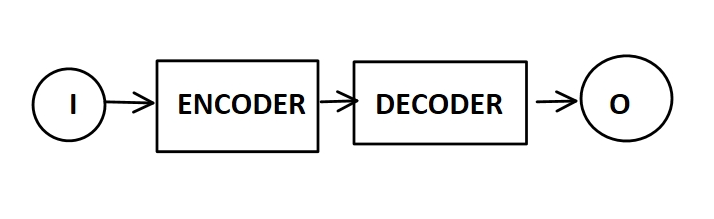
\includegraphics[width=0.8\textwidth]{transformer.png}
    \caption{Mô hình hoạt động của Transformer model}
\end{figure}
\subsection{Language model}
Language model (mô hình ngôn ngữ) là một mô hình được huấn luyện để dự đoán các từ tiếp theo trong một câu nhằm tạo ra các đoạn văn bản mạch lạc, logic và có ý nghĩa. Mô hình này có thể tự viết ra rất đa dạng các thể loại văn bản tùy theo mục đích của người sử dụng. Mô hình đơn giản của language model có thể minh họa như sau:
\begin{figure}[h]
    \centering
    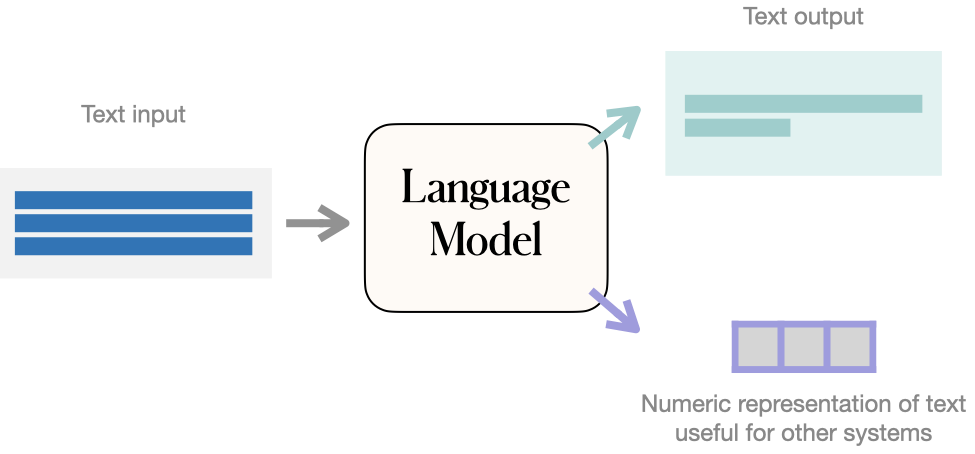
\includegraphics[width=0.8\textwidth]{Cohere-Language-Model.png}
    \caption{Mô hình hoạt động của Language model}
\end{figure}
\section{Nguyên lý hoạt động}
Giả sử khi người sử dụng nhập vào một câu chưa hoàn chỉnh chẳng hạn như "Quantum mechanics is", mô hình sẽ tìm kiếm và dự đoán các từ có khả năng xuất hiện tiếp theo trong output sao cho phù hợp với ngữ cảnh của cả câu văn rồi
thực hiện sắp xếp khả năng xuất hiện của các từ theo xác suất từ cao đến thấp: \cite{link_8}
\begin{itemize}
    \item Quantum mechanics is a...(4.5\%)
    \item Quantum mechanics is based...(3.8\%)
    \item Quantum mechanics is described...(3.2\%)
    \item Quantum mechanics is many...(0.7\%)
\end{itemize}
Sau đó mô hình sẽ lựa chọn giữa các từ "a", "based", "described", "many" để thêm vào trong câu trả lời. Quá trình này sẽ được lặp
lại liên tục cho đến khi câu trả lời được hoàn tất. Thế nhưng không nhất thiết lúc nào mô hình cũng lựa chọn từ với xác suất xuất hiện cao nhất, điều này nhằm tăng thêm tính ngẫu nhiên và sáng tạo của các câu trả lời do AI tạo ra.
Chẳng hạn như thay vì chọn "a" với xác suất cao nhất, AI hoàn toàn có thể lựa chọn "based" để hoàn thành một câu như sau:
\\"Quantum mechanics is based on a set of fundamental principles of morden physics."
\\Qua đây ta có thể thấy rằng AI có thể tạo ra rất nhiều câu trả lời phong phú nhưng vẫn phù hợp với ngữ cảnh.
\section{Quy trình huấn luyện AI}
Để có thể đưa ra các câu trả lời hoàn chỉnh và giống với ngôn ngữ "người" nhất, AI phải trải qua 3 giai đoạn huấn luyện (training) gồm:
\subsection{Giai đoạn 1}
Trong giai đoạn 1, người huấn luyện sẽ đóng cả hai vai trò là người sử dụng (user) và một chatbot lý tưởng (ideal chatbot) và tạo ra các cuộc hội thoại. Thông qua quá trình này, AI có thể học được từ các điểm tương đồng giữa các cuộc hội thoại để từ đó có thể tạo ra các câu trả lời 
gần giống với ngôn ngữ "người" nhất.
\subsection{Giai đoạn 2}
Trong giai đoạn 2, nhà phát triển sẽ "dạy" AI cách để đánh giá hay xếp hạng các output. Chẳng hạn như đối với yêu cầu "Describe an atom.", có 3 output tương ứng và được người huấn luyện xếp hạng như sau:\cite{link_8}
\begin{enumerate}
    \item It's the smallest part of a substance made of protons, electrons and neutrons.
    \item It's a basic chemical element.
    \item It's a ticketing service.
\end{enumerate}
AI sẽ nhận thứ tự sắp xếp theo độ chính xác 1>2>3 và sẽ đưa ra câu trả lời thứ 1 khi được yêu cầu trả lời.
\subsection{Giai đoạn 3}
Ở giai đoạn này, AI có thể tự học thông qua khả năng học tăng cường (reinforcement learning - RF) để có thể xử lý được các câu hỏi ở dạng "mở" như "Write a short story.", loại câu hỏi không có output rõ ràng.
AI đã có thể xử lý một lượng khổng lồ các bài báo, bài viết,... của con người trên internet để tổng hợp, phân tích và tìm các điểm chung giữa chúng để có thể tạo ra câu trả lời hợp lý nhất. Hiện nay, các AI mạnh như ChatGPT còn có khả năng học tăng cường từ các phản hồi của người dùng (reinforcement learning from human feedbacks - RLHF),
điều này càng làm tăng sức mạnh của công cụ trí tuệ nhân tạo.

\chapter{Ứng dụng và tiềm năng phát triển}
\section{Ứng dụng của Copilot}
Cho đến thời điểm hiện tại, Copilot đã được ứng dụng vào trong một số lĩnh vực sau:
\begin{itemize}
    \item Phát triển phần mềm: Copilot được sử dụng để các lập trình viên có thể viết code nhanh và chính xác hơn, điều đặc biệt nhất là Copilot có khả năng debug tốt, giúp cải thiện đáng kể hiệu suất làm việc.
    \item Soạn thảo văn bản: Copilot có thể ứng dụng để soạn thảo các đoạn văn bản từ đơn giản đến phức tạp tùy theo nhu cầu của người sử dụng.
    \item Dịch thuật: khả năng dịch thuật của Copilot tương đối tốt khi có thể dịch trôi chảy giữa các đoạn văn bản phức tạp của các ngôn ngữ khác nhau.
\end{itemize}
Ngoài ra, Copilot đã được tích hợp vào trong các sản phẩm của Microsoft như Office 365 \cite{link_9}. Tiêu biểu như:
\begin{enumerate}
    \item Excel: Copilot hỗ trợ phân tích và truy cập dữ liệu để từ đó có thể đưa ra các phương án tối ưu nhất cho người sử dụng.
    \item Word: Copilot có khả năng viết, chỉnh sửa, tóm tắt, tạo ra các phương án đề xuất và luôn hỗ trợ bên cạnh người dùng.
    \item PowerPoint: Copilot có khả năng tạo một bản powerpoint hoàn chỉnh từ một file word hay một dàn ý cho trước.
    \item Outlook: Copilot hỗ trợ người dùng xử lý các bản nháp, tổng hợp lại các mail quan trọng, phân loại các mail; từ đó người dùng sẽ không mất quá nhiều thời gian trong việc dọn dẹp hòm thư của mình.
\end{enumerate}
\section{Tiềm năng trong tương lai}
Trong tương lai, Copilot có thể phát triển theo các hướng sau:
\begin{enumerate}
\item Cải thiện độ chính xác và hiệu quả: Copilot hiện đang được đào tạo trên một tập dữ liệu khổng lồ gồm mã và văn bản. Khi tập dữ liệu này tiếp tục được mở rộng và cải thiện, Copilot sẽ có thể cung cấp các đề xuất chính xác và hữu ích hơn cho người dùng. Ngoài ra, Copilot cũng có thể được cải thiện về hiệu quả, chẳng hạn như giảm thời gian cần thiết để tạo ra các đề xuất. 
\item Mở rộng khả năng hoạt động: Copilot hiện chỉ hỗ trợ một số ngôn ngữ lập trình và tác vụ. Trong tương lai, Copilot có thể được mở rộng để hỗ trợ nhiều ngôn ngữ lập trình và tác vụ hơn, chẳng hạn như viết tài liệu, dịch ngôn ngữ, v.v. 
\item Thích ứng với người dùng: Copilot hiện đang được đào tạo dựa trên các tập dữ liệu chung. Trong tương lai, Copilot có thể được cá nhân hóa cho từng người dùng, dựa trên sở thích và lịch sử sử dụng của họ. Điều này sẽ giúp Copilot cung cấp các đề xuất phù hợp hơn với nhu cầu của từng người dùng. 
\end{enumerate}

% \bibliographystyle{apacite}
% \bibliography{References.bib}
\begin{thebibliography}{1}
\bibitem{link_1}  \url{https://www.seowebmarketing.co.uk/bing-company-history/}
\bibitem{link_2}  \url{https://techcommunity.microsoft.com/t5/copilot-formerly-bing-chat/copilot-is-the-new-name-for-bing-chat-enterprise/m-p/3984064}
\bibitem{link_3}   \url{https://www.microsoft.com/en-us/edge/features/bing-chat?form=MA13FJ}
\bibitem{link_4}  \url{https://blogs.bing.com/search/may_2023/Bing-Preview-Release-Notes-Chat-History,-Charts,-Export,-and-more} 
\bibitem{link_5}    \url{https://www.microsoft.com/en-us/bing/do-more-with-ai/what-is-bing-chat-and-how-can-you-use-it?form=MA13KP}
\bibitem{link_6} \url{https://youtu.be/4qGrteTY1EM?si=8yITjA6Ddpi42ovW}
\bibitem{link_7} \url{https://youtu.be/ZXiruGOCn9s?si=M-YPdzmx7ityE2gd}
\bibitem{link_8}    \url{https://youtu.be/WAiqNav2cRE?si=ZfTP2cUvpYqezXT4}
\bibitem{link_9} \url{https://www.microsoft.com/en-us/microsoft-copilot#tabs-ocb8dd_tab0}
\end{thebibliography}
\end{document}